\section{商业化：内容公司的三方金字塔}

内容公司的商业化，第一原则是守住三方价值：甲方获得真实有效的品牌表达，创作者愿意为作品署名，观众觉得自己看到了值得信任的内容。Tim 在这一段访谈里把影视飓风的收入说得很直接：广告、商业服务/直播、电商三块构成现金流；真正难的地方在于，钱进入内容之后，内容还要像作品，不能退化成一次投放任务。

\begin{figure}[H]
\centering

\includegraphics[width=0.70\linewidth,height=0.30\textheight,keepaspectratio]{figures/selected/frame_00-59-56_commercialization_question.jpg}
\caption{商业化问题：内容公司绕不开的经营命题。\protect\footnotemark}
\end{figure}
\footnotetext{源时间：00:59:55--01:00:04。}

本章只基于 \texttt{work/segments/segment\_05\_commercialization.md} 与已检查图像写作。源字幕是 AI 中文字幕，个别人名、行业词和口语数字可能存在识别噪声；例如“烧麦老师”这一称呼来自 ASR 文本，本章保守沿用，不扩展源外身份信息；“中药部”等明显误识别按上下文校正为“中腰部”。

\subsection{三块收入：广告、商业服务/直播、电商}

Tim 对商业化的拆分很朴素：影视飓风本质上有三块收入，分别是广告、商业服务或直播业务，以及电商。教学上可以把它理解为同一个影响力资产的三种变现接口：广告出售的是品牌与内容场景的连接，商业服务出售的是创意、制作和直播交付能力，电商出售的是自有产品与长期用户关系。

这三块收入背后有一个共同底座，Tim 称为粉丝经济。粉丝经济的关键，是把长期信任、内容调性和传播能力转化为商业机会；把粉丝当作流量矿，会快速透支账号信用。若用一个简化模型表示：

$$
R = R_{\text{广告}} + R_{\text{服务}} + R_{\text{电商}}
$$

其中：

\begin{itemize}
  \item $R$：内容公司的总收入，表示影响力资产最终形成的现金流。
  \item $R_{\text{广告}}$：品牌投放、商单和内容植入收入。
  \item $R_{\text{服务}}$：全案创意、制作服务、直播业务等项目收入。
  \item $R_{\text{电商}}$：自有产品、衍生品或内容品牌承接的销售收入。
\end{itemize}

这个公式是教学化概括，原访谈没有给出数学表达。它的价值在于提醒读者：内容公司的收入结构看似分散，底层都依赖同一件事，观众是否愿意继续把注意力交给这个账号。

\begin{figure}[htbp]
\centering

\includegraphics[width=0.84\linewidth,height=0.40\textheight,keepaspectratio]{figures/generated/fig_commercialization_paths.pdf}
\caption{商业化路径：广告、商业服务、电商与创意权。此图为教学化整理，综合自 00:59:55--01:02:28 与 01:07:57--01:10:46。}
\end{figure}

\subsection{创意权决定毛利、议价能力与现金流压力}

广告行业有明显上下游。只负责执行拍摄时，内容公司处在可替代位置：甲方或代理公司已经给出创意，制作方主要拼报价、工期和执行稳定性。Tim 的判断更尖锐：如果拿不到创意权，毛利很难上去，垫款压力会迅速吞掉现金流。

这里的“创意权”包含三层含义。第一，内容公司能提出完整方案，甲方收到的是从洞察到表达的整体设计。第二，甲方愿意相信内容团队对观众心理、节奏和传播方式的判断。第三，项目可以在创意确认之后先拿到预付款，减轻差旅、设备、场地、人员等前期支出压力。

现金流压力可以用一个简单式子表示：

$$
P_{\text{现金}} \approx C_{\text{前期支出}} - A_{\text{预付款}} + D_{\text{账期风险}}
$$

其中：

\begin{itemize}
  \item $P_{\text{现金}}$：项目对公司现金流造成的压力。
  \item $C_{\text{前期支出}}$：拍摄前和拍摄中已经发生的支出，包括差旅、设备、场地、人力和后期投入。
  \item $A_{\text{预付款}}$：项目早期收到的预付款，通常来自甲方对方案的认可。
  \item $D_{\text{账期风险}}$：尾款回收时间、审批周期和付款不确定性带来的风险。
\end{itemize}

这个模型能解释 Tim 为什么强调创意权。创意权带来的好处会进入公司的财务结构：预付款越早进入，垫款越少；毛利越高，试错空间越大；甲方越信任方案，团队越能把商业内容做成作品。

\begin{knowledgebox}{背景解释：毛利与垫款}
毛利可以粗略理解为项目收入扣除直接成本后的剩余空间。垫款指公司先替项目把钱花出去，后续再等甲方付款。内容项目常有差旅、设备、人员和后期成本，若毛利低且回款慢，公司看上去接了不少单，账上现金却会被前期支出抽空。
\end{knowledgebox}

\subsection{科沃斯点云故事：商业内容如何同时成立}

科沃斯扫地机器人案例，是本章最关键的商业内容样本。按 Tim 的叙述，影视飓风早已有一个创意：艺术家烧麦老师希望纪念离世的爷爷，想把爷爷的房间留下来；团队需要扫描房间、采集数据，甚至涉及武汉城市空间与点云视觉表达。科沃斯的扫地机器人激光雷达，正好能被真实地用于这个创意。

这个项目的价值在于三条线同时成立。对甲方来说，设备能力被真实使用，品牌露出只占表层；对创作者来说，这个故事有情感、有技术挑战，也有艺术表达空间；对观众来说，内容的主体验是纪念、点云可视化与人的情感，口播退到辅助位置。

\begin{importantbox}{三方商业内容原则}
商业内容要同时回答三个问题：

\begin{itemize}
  \item 甲方是否满意：产品能力、品牌信息和合作目标是否被清楚表达。
  \item 创作者是否热爱：团队是否愿意把审美、技术和情感投入到项目里。
  \item 观众是否喜欢：观众是否获得故事、知识、情绪或审美价值，并愿意承认这是一条好内容。
\end{itemize}

三方价值同时成立时，商业内容才有机会从“投放”升级为“作品”。其中任何一方长期受损，账号的信任资产都会被消耗。
\end{importantbox}

这个三角关系也解释了为什么自媒体商业内容比传统 TVC 更复杂。传统广告的验收重心通常落在甲方，甲方点头意味着交付结束；自媒体账号还要面对观众，观众会把商业内容直接记在创作者身上。商业内容如果让观众感觉被糊弄，伤害会回到账号长期信用。

\begin{warningbox}{风险：观众信任一旦损坏，商业效率会反向下降}
观众信任像账户本金。短期商业化可以提高当期收入，粗糙植入、虚假体验和低质量口播会消耗本金。本金下降之后，广告报价、转化率、评论区氛围和下一条内容的首轮传播都会受影响。对内容公司来说，失去观众信任会从单次项目事故扩大成资产负债表上的隐性亏损。
\end{warningbox}

\subsection{承认昂贵内容失败：创作伦理也要看结果}

Tim 在这一段把话说得很狠：有些内容投入几十万、做了两个月，播放量只有七八十万，没有达到共鸣目标，他会直接判定这期内容失败。这里讨论的是结果责任：播放量只是信号，内容公司真正要面对的是目标有没有达成。团队很辛苦，成本很高，周期很长，这些都无法自动换成观众共鸣。

这条标准对创作者很残酷，也很必要。内容公司最容易给自己找借口：项目难、预算大、团队努力、技术复杂、甲方满意。Tim 的标准把这些理由压回同一个问题：作品有没有打动人，目标有没有达成，观众有没有被说服。

商业闭环也有危险性。访谈中刘润追问：好内容吸引品牌，品牌收入支持好内容，理论上这是一个正循环。Tim 随即指出，这里面没有稳定的直接因果关系。内容做得好，品牌预算也可能收缩；平台分发可能改变；行业投放偏好可能转向直播带货。教学上可以写成：

$$
L_{\text{闭环}} = Q_{\text{内容}} \times B_{\text{品牌预算}} \times S_{\text{平台分发}} \times T_{\text{观众信任}}
$$

其中：

\begin{itemize}
  \item $L_{\text{闭环}}$：商业闭环的强度。
  \item $Q_{\text{内容}}$：内容质量与共鸣能力。
  \item $B_{\text{品牌预算}}$：品牌方可用于投放或合作的预算。
  \item $S_{\text{平台分发}}$：平台算法、流量结构和商业生态带来的分发能力。
  \item $T_{\text{观众信任}}$：观众对账号的长期信任。
\end{itemize}

乘法模型的直觉很简单：任何一个变量大幅降低，闭环都会变弱。这个模型是作者的教学化总结，源访谈提供的是“没有直接因果关系”和“行业风险”这两条判断。

\subsection{平台风险：里世界、外世界与头部效应}

Tim 用“里世界”和“外世界”解释平台风险。类比来自游戏：玩家在游戏内部打装备、做代练，装备看起来有价格；游戏厂商更新规则之后，原来的装备可能立即贬值。创作者在视频平台里也类似。账号看起来有粉丝、有播放、有商业合作，但上面还有平台规则、推荐机制、广告生态和品牌预算。

\begin{figure}[H]
\centering
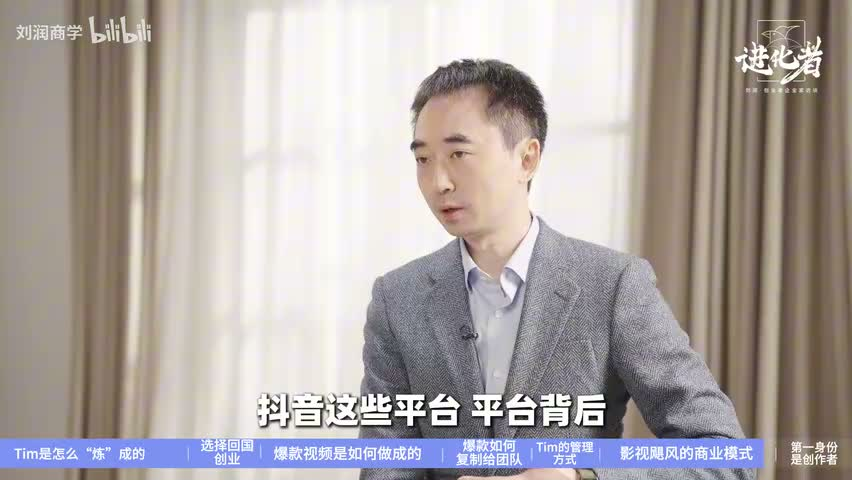
\includegraphics[width=0.70\linewidth,height=0.30\textheight,keepaspectratio]{figures/selected/frame_01-10-00_platform_budget_context.jpg}
\caption{平台和品牌预算变化会改变创作者处境。\protect\footnotemark}
\end{figure}
\footnotetext{源时间：01:09:58--01:10:10。}

这就是中腰部创作者的压力来源。Tim 认为，中腰部博主话语权更小，平台波动会对他们产生巨大影响；品牌总体投放预算减少时，头部账号的预算相对更容易被保护，中腰部批量投放则会优先承压。再加上直播带货把一部分预算拉走，品牌会问一个很现实的问题：中腰部内容投放的转化和认知强化，是否比直播带货更有效？

头部效应因此会越来越强。头部账号既有更高确定性，也能吃到更多预算；更多预算带来更大项目和更强影响力，影响力又让品牌进一步集中。经济学里常把这种现象叫马太效应：已有优势会继续吸附资源。Tim 在 ASR 文本中提到头部可能吃掉很高比例的行业预算，这里应把它理解为口语化的集中度判断；数字层面需要后续人工核验。

\begin{knowledgebox}{概念解释：里世界、外世界与马太效应}
“里世界”指创作者依赖的平台内部生态，包括算法、流量规则、商业产品和推荐机制。“外世界”指平台之外更大的经济环境，包括品牌预算、消费周期、广告市场和技术变化。马太效应描述资源向已有优势者集中的现象，可用一句话概括：越有影响力，越容易获得下一轮影响力资源。
\end{knowledgebox}

\subsection{本章小结}

本章的核心结论是：内容公司的商业化能力，取决于现金流结构、创意权、观众信任和平台环境共同作用。

\begin{itemize}
  \item 收入层面，广告、商业服务/直播、电商是三块主要现金流，底层都依赖粉丝经济与长期信任。
  \item 议价层面，创意权决定内容公司能否摆脱低毛利执行位置，并通过预付款缓解垫款压力。
  \item 作品层面，科沃斯激光雷达点云案例说明，商业内容要让甲方、创作者和观众三方同时获得价值。
  \item 伦理层面，高成本内容没有天然荣誉，结果失效就要承认失败；这是一种对观众、团队和商业伙伴负责的标准。
  \item 风险层面，平台规则、品牌预算转移、直播带货替代、中腰部压力和头部效应，会持续改变内容公司的商业边界。
\end{itemize}

读者应带走一个判断：商业化是内容理想进入现实约束后的经营系统，它会反过来塑造内容选题、制作尺度、组织现金流和账号信任。真正可持续的内容公司，需要在赚钱时仍然证明自己值得被看见、被相信、被传播。
